%%%%%%%%%%%%%%%%%%%%%%%%%%%%%%%%%%%%%%%%%%%%%%%%%%%%%%%%%%%%%%%%%%%%%%%%%%%%%%
% CS240: Programming in C
% Copyright 2016 Pejman Ghorbanzade <mail@ghorbanzade.com>
% Creative Commons Attribution-ShareAlike 4.0 International License
% https://github.com/ghorbanzade/UMB-CS240-2016S/blob/master/LICENSE
%%%%%%%%%%%%%%%%%%%%%%%%%%%%%%%%%%%%%%%%%%%%%%%%%%%%%%%%%%%%%%%%%%%%%%%%%%%%%%

\def \topDirectory {.}
\def \resDirectory {\topDirectory/src/c/main/ls03}
\def \texDirectory {\topDirectory/src/tex}
\def \styDirectory {\texDirectory/sty}
\def \cfgDirectory {\texDirectory/cfg}
\def \imgDirectory {\texDirectory/img}

\documentclass[compress]{beamer}
%\mode<presentation>
%\usetheme{default}

\usepackage{\styDirectory/directives}
%%%%%%%%%%%%%%%%%%%%%%%%%%%%%%%%%%%%%%%%%%%%%%%%%%%%%%%%%%%%%%%%%%%%%%%%%%%%%%
% CS114: Introduction to Programming in Java
% Copyright 2015 Pejman Ghorbanzade <mail@ghorbanzade.com>
% Creative Commons Attribution-ShareAlike 4.0 International License
% https://github.com/ghorbanzade/UMB-CS114-2015F/blob/master/LICENSE
%%%%%%%%%%%%%%%%%%%%%%%%%%%%%%%%%%%%%%%%%%%%%%%%%%%%%%%%%%%%%%%%%%%%%%%%%%%%%%

\course{id}{CS240}
\course{name}{Programming in C}
\course{venue}{Mon/Wed, 5:30 PM - 6:45 PM}
\course{semester}{Spring 2016}
\course{department}{Department of Computer Science}
\course{university}{University of Massachusetts Boston}

\instructor{name}{Pejman Ghorbanzade}
\instructor{title}{}
\instructor{position}{Student Instructor}
\instructor{email}{pejman@cs.umb.edu}
\instructor{phone}{617-287-6419}
\instructor{office}{S-3-124B}
\instructor{office-hours}{Mon/Wed 16:00-17:30}
\instructor{address}{University of Massachusetts Boston, 100 Morrissey Blvd., Boston, MA}

\usepackage{\styDirectory/beamerthemePejman}
\doc{number}{3}
%\setbeamertemplate{footline}[text line]{}

\begin{document}

\prepareCover

\section{Introduction to C}

\begin{slide}
	\begin{columns}
	\column{0.4\textwidth}
	\begin{block}{Motivation}
	Developed in 1972 to re-implement Unix operating system for PDP-11.
	\end{block}
	\column{0.6\textwidth}
	\begin{figure}
	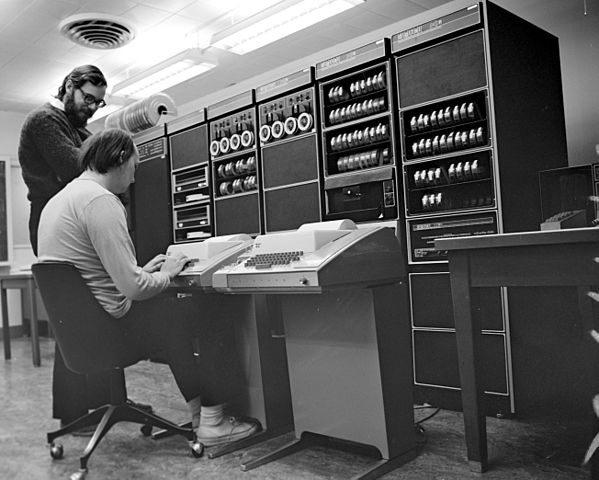
\includegraphics[width=0.8\textwidth]{\imgDirectory/pioneers.jpg}
	\end{figure}
	\end{columns}
\end{slide}

\begin{slide}
	\begin{block}{Features}

	\begin{itemize}
	\item[] Portable
	\item[] Small
	\item[] Fast
	\item[] Powerful
	\end{itemize}

	\end{block}
\end{slide}

\begin{slide}
	\begin{block}{Popularity of C}

	\begin{figure}
	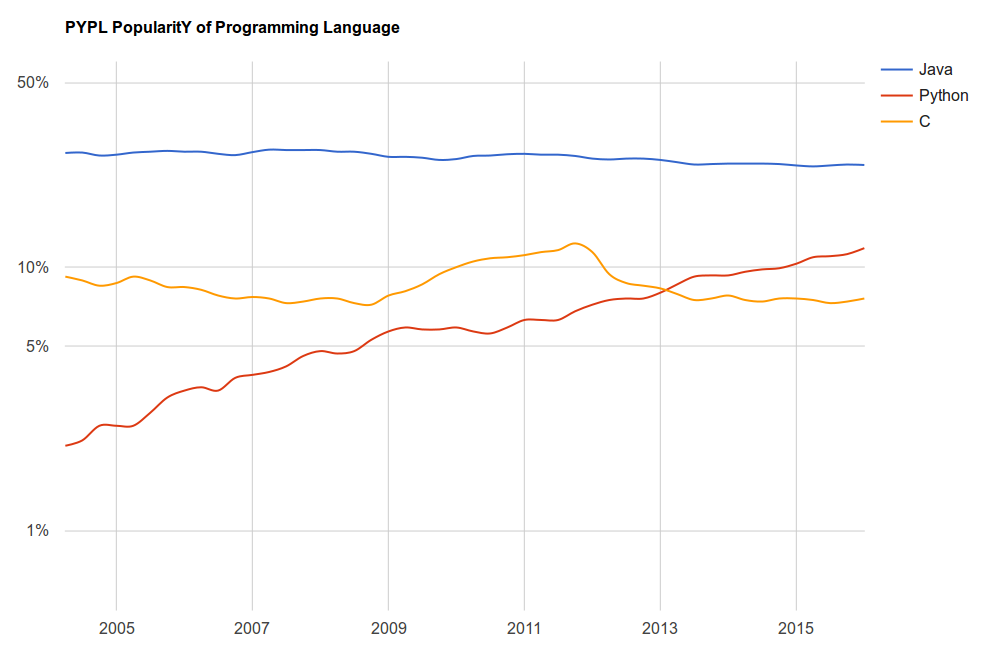
\includegraphics[width=0.8\textwidth]{\imgDirectory/pypl.png}
	\end{figure}

	\end{block}
\end{slide}

\begin{slide}
	\begin{block}{Hello World Program}

	\inputminted[
		fontsize=\scriptsize,
		firstline=10,
		linenos
	]{c}{\resDirectory/hello-world.c}

	\end{block}
\end{slide}

\begin{slide}
	\begin{block}{Running Hello World Program}

	\begin{terminal}
	pejman@cs240:~$ pwd
	/home/pejman
	pejman@cs240:~$ mkdir hello
	pejman@cs240:~$ cd hello
	pejman@cs240:~/hello$ touch hello-world.c
	pejman@cs240:~/hello$ vi hello.c
	pejman@cs240:~/hello$ gcc hello.c
	pejman@cs240:~/hello$ ls
	a.out   hello.c
	pejman@cs240:~/hello$ ./a.out
	Hello World!
	\end{terminal}

	\end{block}
\end{slide}

\begin{slide}
	\begin{block}{GNU Compiler Collection}

	Originally named GNU C Compiler, \alert{\texttt{gcc}} is the compiler system of GNU project that supports C, C++, Objective C, Java, Ada and Go.

	\end{block}
	\begin{block}{Other C Compilers}

	\begin{itemize}
	\item[] clang
	\item[] MinGW
	\end{itemize}

	\end{block}
\end{slide}

\begin{slide}
	\begin{block}{Comments}

	Any character between \alert{\texttt{/*}} and \alert{\texttt{*/}} is ignored by the compiler.

	\inputminted[
		fontsize=\small,
		firstline=13,
		lastline=15
	]{c}{\resDirectory/comment.c}

	Any character after \alert{\texttt{//}} in a line is considered a comment and is ignored by the compiler.

	\inputminted[
		fontsize=\small,
		firstline=18,
		lastline=18
	]{c}{\resDirectory/comment.c}

	\end{block}
\end{slide}

\begin{slide}
	\begin{block}{Preprocessor Directives}

	source lines of code preceded by a hash sign (\#) are directives for C preprocessor.

	\inputminted[
		fontsize=\scriptsize,
		firstline=10,
		lastline=11
	]{c}{\resDirectory/comment.c}

	\alert{\texttt{\#include}} directive appends a specified header file to the current file.

	\end{block}
\end{slide}

\begin{slide}
	\begin{block}{Functions}

	A \alert{function} is a set of statements enclosed in braces \{\} with a \emph{unique} name that is followed by a parenthesized list of arguments.
	A function may \emph{return} a value of a specific data type.

	\end{block}
\end{slide}

\begin{slide}
	\begin{block}{The \texttt{main} function}

	Each C program must have a function named \texttt{main}.
	A C program terminates when all statements inside its \texttt{main} function are executed.

	\inputminted[
		fontsize=\small,
		firstline=12,
		linenos
	]{c}{\resDirectory/hello-world.c}

	\end{block}
\end{slide}

\begin{slide}
	\begin{block}{Statements}

	A statement is a command that instructs the computer to take a specific set of actions.
	All statements must end with a semicolon.

	\inputminted[
		fontsize=\small,
		firstline=14,
		lastline=14
	]{c}{\resDirectory/hello-world.c}

	\end{block}
\end{slide}

\begin{slide}
	\begin{block}{\texttt{printf} Function}

	\texttt{printf} function formats a string with given arguments and sends the formatted string to standard output.
	\texttt{printf} function is part of \texttt{stdio} library and is defined in \texttt{printf.c} file.

	\inputminted[
		fontsize=\small,
		firstline=13,
		lastline=21,
		linenos
	]{c}{\resDirectory/printf.c}

	\end{block}
\end{slide}

\begin{slide}
	\begin{block}{Put Your Knowledge Into Practice}

	\begin{figure}
	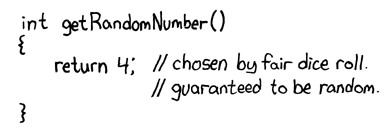
\includegraphics[width=0.8\textwidth]{\imgDirectory/random.png}
	\end{figure}

	\end{block}
\end{slide}

\end{document}
